\chapter[Introdução]{Introdução} \label{cap:introducao}
% \addcontentsline{toc}{chapter}{Introdução}

A democracia digital é resumida por \citeonline{penteadoencontro} como o uso da Internet para consolidação da democracia.
Este uso tem acarretado um crescente número de discussões acerca de temas políticos, 
o que permitiu que interessados na área analisassem esse fenômeno e observassem uma 
polarização das mensagens trocadas nas redes sociais \cite{empurrandojuntos}.

\citeonline{empurrandojuntos} afirmaram que as discussões realizadas, principalmente em redes sociais, 
acabavam refletindo sempre a opinião da maioria e que as pessoas estão sempre presentes em uma bolha de opinião. 
Isto é, os algoritmos dessas plataformas selecionam o conteúdo a ser apresentado de acordo com o comportamento anterior,
no qual foi coletada a opinião deste usuário.
Dessa forma, essa polarização dificulta a explanação das ideias da minoria e restringe a apresentação de 
pensamentos diferentes para quem usa essas redes sociais. 

Observando esse aspecto, o Instituto Cidade Democrática\footnote{Site do Cidade Democrática: \url{http://www.cidadedemocratica.org.br/}} 
apresenta a plataforma ``Empurrando Juntos'' cujo objetivo 
é dar voz para a minoria e tornar as discussões mais efetivas para os seus propósitos \cite{empurrandojuntos}.

A ideia é que um usuário entre em um \textit{website} ou em um aplicativo de celular para criar conversas e 
participar de conversas criadas por outros usuários. Essa participação 
acontece de duas formas: comentando uma conversa ou votando em um comentário de outro participante. Entende-se por voto
o ato de concordar com o comentário realizado (uma espécie de \textit{like}) ou discordar do comentário. Além disso, é permitido
que o usuário pule aquele comentário, ou seja, não atribua nenhum tipo de voto \cite{empurrandojuntos}. 

Com os votos realizados, é possível agrupar pessoas que responderam de maneira parecida, ou seja, concordaram e
discordaram dos mesmos comentários. Com os grupos formados, é possível ver a convergência e divergência de opiniões, 
prover ao usuário uma visão ampliada acerca do assunto e promover a interação entre os usuários com 
pensamentos divergentes. A Figura \ref{fig:resumo_ej} ilustra o funcionamento completo do sistema.

\begin{figure}[h!]
\centering
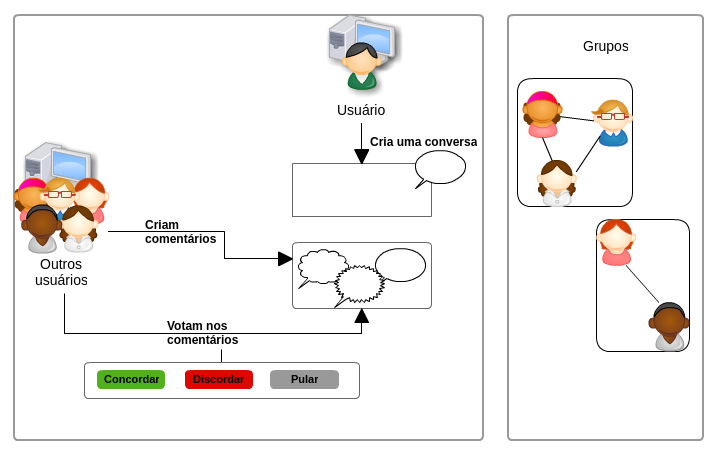
\includegraphics[scale=0.6]{figuras/resumo_ej.png}
\caption{Funcionamento do ``Empurrando Juntos''}
\label{fig:resumo_ej}
\end{figure}

Os usuários interagem com as conversas e o sistema é responsável por agrupá-los de acordo com essa interação.
Observa-se que o sistema é dividido em dois processamentos: gestão de usuários 
e conversas (conversas, comentários e votos) e agrupamento de pessoas com base em seus votos. 

Este agrupamento deve ser realizado em tempo real, ou seja, conforme as pessoas votam os grupos são formados ou modificados. 
Portanto, não há estabelecimento prévio dos grupos, são conhecidos apenas os dados em comum entre os usuários, que são os votos nas conversas. 
Desta maneira, esta formação de grupos pode ser executada utilizando técnicas de classificação,
pois essas técnicas, de acordo com \citeonline{tan2013data, han2011data, clustering_review} , 
têm como objetivo encontrar um modelo que possa descrever e distinguir classes de dados.
Sendo assim, nota-se a necessidade de um processo de classificação para que esses grupos sejam formados. 

Existem diversas técnicas de classificação que podem ser utilizadas no contexto do ``Empurrando Juntos'', uma delas é a
clusterização que, de acordo com \citeonline{tan2013data, clustering_review}, é uma técnica utilizada para agrupamentos 
nos quais os rótulos não necessitam ser definidos. Além da diversidade de métodos de classificação, a própria clusterização pode ser implementada com o uso de 
diferentes técnicas e algoritmos. 

Considerando os dois processamentos envolvidos, a possibilidade do uso de diferentes técnicas para a 
realização do agrupamento e a característica do ``Empurrando Juntos'' de ser uma aplicação multiplataforma, notou-se
a necessidade do estabelecimento de uma arquitetura em três módulos: servidor, cliente e matemático. Na qual, o módulo servidor 
consistiria em uma \textit{Application Programming Interface} (API) que, de acordo com \citeonline{wagh2012comparative, understanding_web}
é uma interface que expõe os seus componentes como um serviço, permitindo que outras aplicações interajam com esses 
componentes. Desse modo, possibilita o compartilhamento dos dados armazenados com as aplicações que a consomem.

A parte cliente da aplicação seria responsável pela interface visual e comunicação com a parte servidor no processamento
de usuários e ações no sistema. E o módulo matemático teria a finalidade de formar os grupos de pessoas de acordo com os votos realizados.

Dessa forma, o objetivo do trabalho foi estabelecer a arquitetura do ``Empurrando Juntos'' e implementar
o módulo de API, permitindo a utilização de diferentes plataformas para o módulo cliente e diferentes algoritmos para o módulo matemático.

Para realização do objetivo proposto, o trabalho foi dividido em cinco etapas, conforme a Figura \ref{fig:etapas_trabalho}. 

\begin{figure}[h!]
\centering
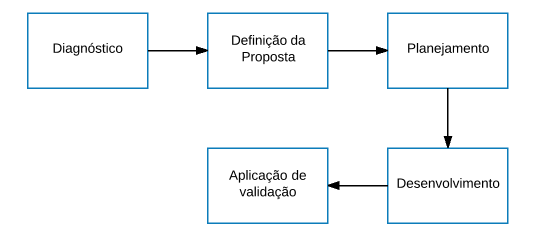
\includegraphics[scale=0.6]{figuras/etapas.png}
\caption{Etapas do trabalho}
\label{fig:etapas_trabalho}
\end{figure}

A etapa de ``Diagnóstico'' compreendeu o entendimento do escopo da plataforma ``Empurrando Juntos''. 
A etapa de ``Definição da Proposta'' foi caracterizada pela definição de escopo, 
da arquitetura da API e da comunicação com os módulos matemáticos. Na terceira etapa, 
foi feito o planejamento da execução do trabalho com o estabelecimento
de um cronograma das atividades das próximas etapas. 

Na etapa de ``Desenvolvimento'' foram realizadas as iterações de implementação, teste e adaptação da API. 
Por fim, na etapa de ``Aplicação em um caso'' a API foi utilizada em uma plataforma de exemplo em comunicação com os outros dois módulos: cliente e matemático.

Nesse contexto, este trabalho, além desta introdução, está organizado em outros quatro capítulos. 
O Capítulo \ref{cap:clusterizacao} aborda os conceitos e técnicas de 
classificação, com foco na técnica utilizada no módulo matemático implementado. 
A solução proposta no trabalho é apresentada no Capítulo \ref{cap:proposta}. No Capítulo \ref{cap:aplicacao_exemplo} é
apresentado o caso de exemplo do uso da API. E por fim são apresentadas as conclusões no Capítulo \ref{cap:consideracoes_finais}.
